\documentclass[]{article}
\usepackage{graphicx}
\usepackage[a4paper,margin=1in,footskip=0.25in]{geometry}
\usepackage{float}
\usepackage[parfill]{parskip}
\graphicspath{ {./images/} }

%opening
\title{}
\author{}

\begin{document}
	
\maketitle

\section{Introduction}

\subsection{Markov Decision Process}

A Markov chain is a stochastic model meaning that it randomly determined process. The chain describes a sequence of possible events in which the probability of each event depends only on the state attained in the previous event. 

\begin{figure}[H]
	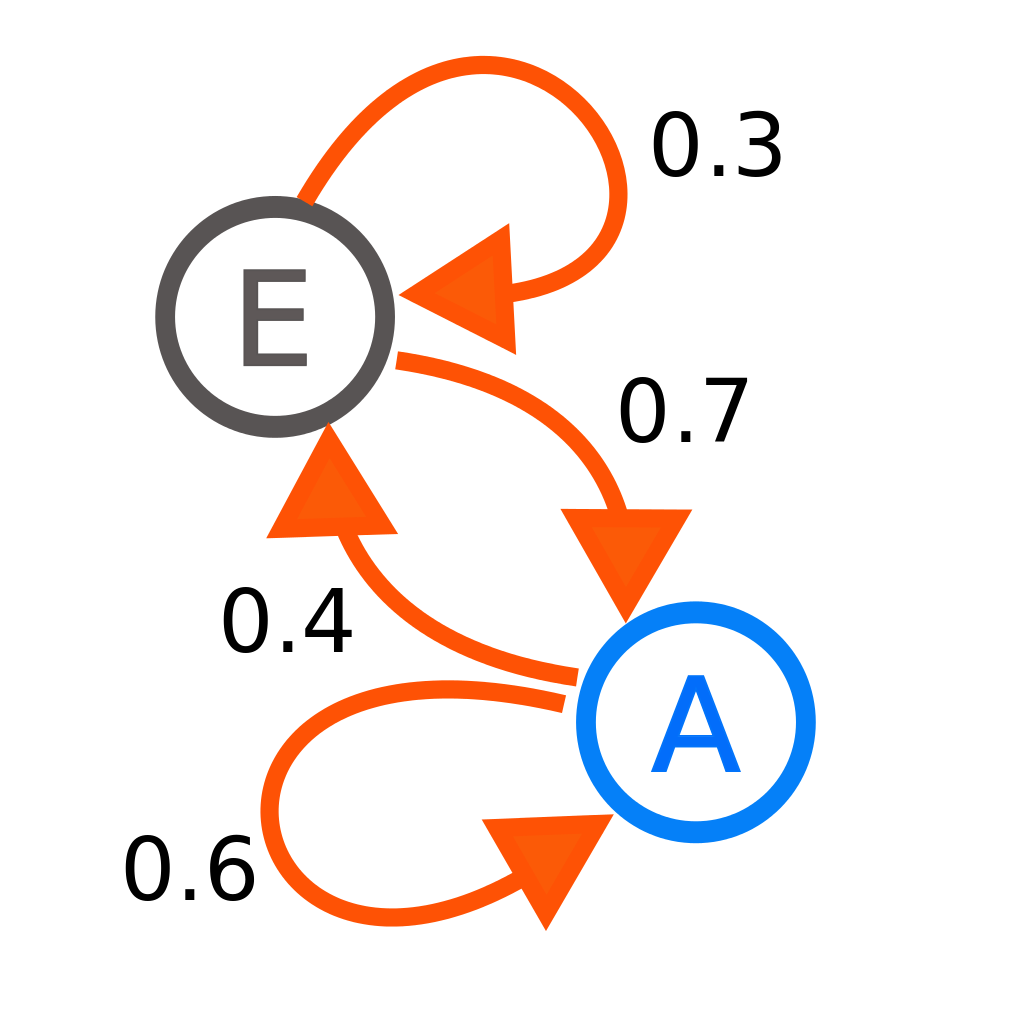
\includegraphics[scale=0.1]{markov}
	\centering
	\caption{A two-state Markov process.}
\end{figure}

A Markov decsion process is a discrete time stochastic control process. Markov decision processes provide a mathematical framework for modelling decision making in situations where outcomes are partly random and partly under the control of a decision maker. A stochastic process has the Markov property if the conditional probability distribution of future states of the process depends only upon the present state, not on the sequence of events that preceded it. A process with this property is called a Markov process.

At each time step, the process is in some state $s$ and the decision maker may choose any action $a$ that is available in state $s$. The process responds at the next time step by randomly moving into a new state $s'$ and giving the decision maker's a corresponding reward $R_a(s, s')$.

The probability that the process moves into its new state $s'$ is influenced by the chosen action. It is given by the state transition function $P_a(s, s')$. The next state $s'$ depends on the current state $s$ and the decision maker's action $a$. But given $s$ and $a$, it is conditionally independent of all previous states and actions and therefore satisfies the Markov property. 

\subsection{Reinforcement Algorithm}

\subsection{Q-Learning}

Q-learning is a model free reinforcement algorithm. In q-learning, there is one q value for each possible action you could take given a state.

\section{Implementation}

The agent will try and find the closest route from any square to square 6. The possible states are $S=0,1,2,3,4,5,6,7,8$ and the possible actions are $A=0,1,2,3,4,5,6,7,8,9$. A reward of 1 will be given to the agent if a state is directly reachable from the current state. The search state square 6 will have a reward of 999.

\begin{figure}[H]
	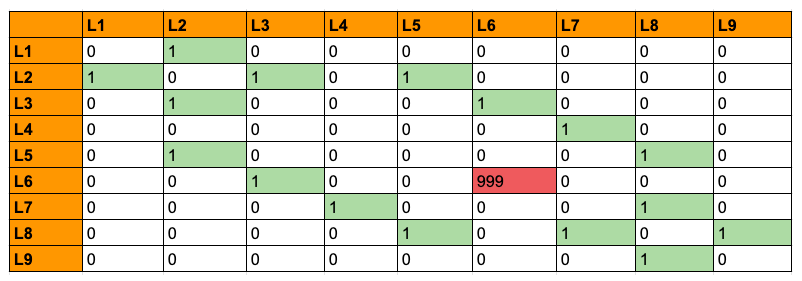
\includegraphics[scale=0.4]{rewards}
	\centering
	\caption{Reward table.}
\end{figure}

\end{document}